\chapter{Testing Tribler at a Large Scale}
\label{chapter:large-scale-experiment}
In the previous chapter, we performed various small performance measurements and quantified the usability and performance of common performed operations in Tribler. While these experiments gave us insights in the performance of key components, we focused on a single part of the system in every experiment.\\\\
In this chapter, we focus on how several components present in Tribler work together. We will perform a test on a large scale, where we start the application, perform a remote keyword search, select a torrent and start a download using the anonymous overlay network. We will first discuss the set-up of the experiment in more detail, after which we turn our focus to the results we observed during the experiment. As far as we aware, this is the first time that we assess the performance of Tribler in general by performing an extensive sequence of operations.

\section{Environment Specifications}
We utilized the DAS5 supercomputer for this test to be able to run several Tribler sessions in parallel. We created a separate job in our CI environment where we allocate ten nodes on the DAS5 \emph{Vrije Universiteit (VU)} cluster every time the job is executed. A summary of hardware specifications of each DAS5 node is presented in Table \ref{table:das5-node-specifications}. On each node, we start exactly one Tribler session.

\begin{table}[h!]
	\centering
	\begin{tabular}{|l|l|}
		\hline
		\emph{CPU} & dual 8-core 2.4 GHz (Intel Haswell E5-2630-v3)\\ \hline
		\emph{Memory} & 64GB \\ \hline
		\emph{Hard disk} & 128TB \\ \hline
		\emph{Operating system} & CentOS Linux \\ \hline
	\end{tabular}
	\caption{The specifications of a node in the DAS5 VU cluster.}
	\label{table:das5-node-specifications}
\end{table}

\section{Set-up of the Experiment}
The experiment as performed in this chapter is structured as follows: we run a specific Tribler scenario 2.172 times on the DAS5 supercomputer and keep track of the timestamps of interesting events during each run. We write this data to a file after each run and combine the results when all nodes in the DAS5 cluster are finished. Since execution of the Jenkins job yields ten results, we repeated the execution of the job multiple times.\\\\
For every running Tribler session, we perform the following operations: first, we start Tribler with a clean state directory, without any prior information about the network. After Tribler has been started, we wait for a sufficient amount of peer  connections (30) in the \emph{SearchCommunity} before we perform the remote search. This is different from the value used in the experiment described in Section \ref{sec:remote-content-search-experiment}, where we wait until we are connected to at least 20 peers. In our experiment, this number has been increased since there are running ten other Tribler nodes inside the same network that are possibly connecting with each other. When this happens, they provide no remote search results to each other since there is likely to be no discovered content in their databases yet. In each Tribler session, we scheduled a check that is executed every second to verify whether we are connected to a sufficient amount of peers.\\\\
Once there are enough established connections, a remote torrent keyword search is performed. For this purpose, we are using a list of 1.000 popular keywords that have been determined as follows: we analysed a database with just over 100.000 torrents, gathered all keywords in the database together with the frequency of each keyword and created a list of the 1.000 keywords with the highest frequency. Every run, we pick a random keyword  with a uniform distribution from this list and perform a remote search with the selected keyword.\\\\
After performing the remote search, we wait 30 seconds for incoming search results to arrive. The time of the first and the last incoming remote search results are tracked, like in the experiment described in Section \ref{sec:remote-content-search-experiment}. If we have no search results within 30 seconds, we mark the run as failed and stop the Tribler session. We save all incoming torrent search results and when the remote search is done, we pick five random, non-explicit torrent results and schedule a meta info lookup in the DHT. We are using a time out period of 60 seconds for the DHT lookup operation: if we do not receive any response from one of the scheduled DHT lookup after this time out period, we mark the run as failed.\\\\
As soon as the first meta info response is received, we start the download of the torrent associated with the meta info. During the download, one hop anonymity is used. Three minutes after initiating the torrent download, we stop the Tribler session and remove the downloaded data. We keep track of the duration of circuit construction and the moment in time when we receive the first incoming content bytes. Additionally, we keep track of the total number of downloaded bytes after these three minutes. A summary of the performed actions during each Tribler run is displayed in Figure \ref{fig:big-experiment-setup}.\\

\begin{figure}[!h]
	\centering
	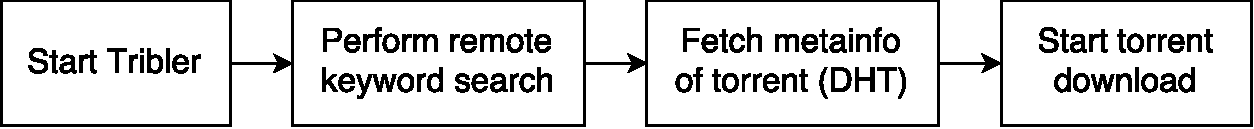
\includegraphics[width=0.7\columnwidth]{images/big_experiment/big_experiment_setup}
	\caption{The actions performed in each run of the experiment described in this chapter.}
	\label{fig:big-experiment-setup}
\end{figure}

We emphasize that this experiment is performed using the real Tribler network and we are not using an artificial environment. The selected torrents for the  download operations are selected in a random matter and we are not selecting these torrents based on the health of the swarm.\\\\
To make the experiment succeed, we had to implement a workaround for a bug in Tribler: after starting an anonymous download in Tribler, the download does not receive any bytes when the circuits have been created. In order to make sure that the download proceeds correctly, we forced start the download after the circuits have been established.

\section{Failure Identification}
We can think of various failures during each run of Tribler, failures that can be classified as code-level defects (which should be recognized by the unit tests) and failures that are attributed to external dependencies such as the health of the swarm or the state of the Tribler network. Below, we summarize some failures:
\begin{itemize}
	\item There is not a sufficient amount of established connections in the \emph{SearchCommunity} after two minutes.
	\item There are no search results after 30 seconds after performing a remote search.
	\item We do not receive a response containing meta info of a torrent within 60 seconds after scheduling five DHT meta info lookup.
	\item Three minutes after the download started, we did not built enough circuits yet.
	\item Three minutes after the download started, we did not receive any content bytes yet.
\end{itemize}
We abort the Tribler session if one of the first three described failures above is observed. We should note that most of these failures can be addressed to the state of the Tribler network. By performing the run as described in the previous Section numerous times, we get insights in the most common failures.

%The order of operations as performed in this experiment is visible in Figure \ref{fig:big-experiment-setup}. The experiment itself is executed on the DAS5 supercomputer where in every run, we allocate ten nodes and run one Tribler instance on every node.\\

%There are various failures that could lead to an interruption of the experiment, which we will summarize below:
%\begin{itemize}
%	\item If we are not connected to at least 30 peers in the \emph{SearchCommunity} after Tribler has started, we abort the experiment.
%	\item If we do not receive any remote torrent result within 30 seconds, we abort the experiment.
%	\item If we do not receive a response from any scheduled DHT lookup, we abort the experiment.
%\end{itemize}
%We also have various failures that influences our result but are not failing our experiment. An example of these failures is when we fail to build circuits within three minutes after starting the download. In this situation, we are still able to finish the experiment, however, our final results are influenced since we were not able to download any byte.

\section{Observed Results}
We will now discuss the results that are obtained during this large-scale experiment. The focus will be both on the amount and distribution of failures that occurred during the experiment and on the duration of the performed operations.

\subsection{Failure Rates}
After performing the experiment, we observed a success rate of 54.2\% which means that in this percentage of the runs, all operations were successful and that we downloaded one or more content bytes. In 45.8\% of the runs, we encountered an issue during the Tribler run. The exact distribution of observed outcomes of the 2.171 runs is presented in Figure \ref{fig:big-experiment-outcome-pie}.

\begin{figure}[!h]
	\centering
	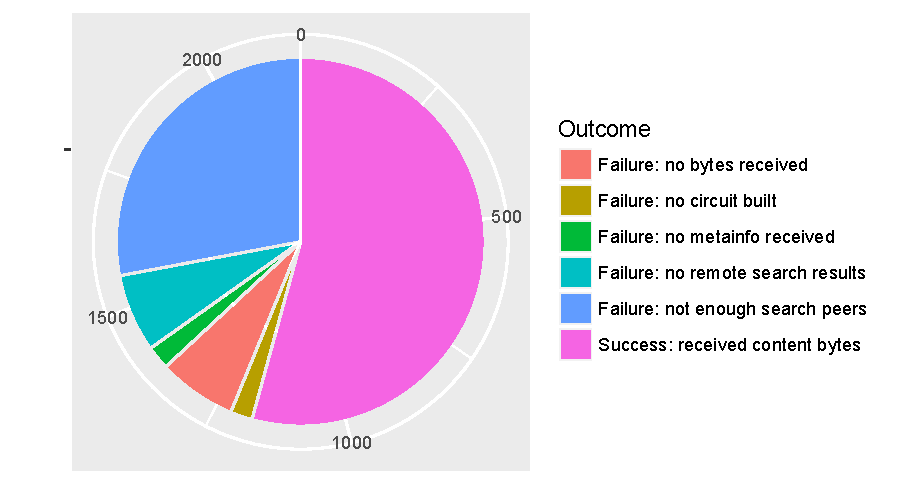
\includegraphics[width=0.7\columnwidth]{images/big_experiment/outcome_pie}
	\caption{The distribution of outcomes of all 2.171 runs.}
	\label{fig:big-experiment-outcome-pie}
\end{figure}

Over half of the runs are succeeding, however, a significant amount of the failures is addressed to the situation where Tribler did not connect to enough peers in the \emph{SearchCommunity} two minutes after start-up (to be exact, in 27.9\% of the runs). If this failure occurred during a run, we recorded the amount of peers that are connected after two minutes and we noticed that this amount often between 20 and 30 peers. This indicates that this failure is not significant anymore if we decide to lower the amount of peers required when searching and that it might have been better if we reduced the required amount of peers. However, by having less connections to remote peers when performing a search, we might lower the quality of search results.\\\\
In 6.9\% of the runs, we did not receive remote search results after 30 seconds. While this result contradicts our findings in the experiment explained in Section \ref{sec:remote-content-search-experiment} (where all our queries resulted in at least one search result), we should emphasize that there might be keywords in our constructed query list that have an unevenly distribution amongst peers. In the database we used to construct the query list, we were subscribed to various channels, having access to an extended amount of content. Connected peers in the search overlay might not have discovered as many torrents as we have, possibly because they are subscribed to fewer channels. This way, the chance for a peer to have content matching a specific keyword, decreases. Another explanation might be that there is a torrent with many files that contains a rare keyword in a significant part of these files. Our selection algorithm will consider this keyword as frequent in the database, however, the torrent file might be new in which case not many peers might know about this torrent.\\\\
In 2.1\% of all runs, we did not receive torrent meta info after scheduling five DHT lookups. In the experiment performed in Section \ref{subsec:dht-experiment}, we concluded that 48.9\% of the scheduled lookups in the DHT failed (with a time out period of 30 seconds). When scheduling five parallel lookups, we estimate that the chance of no request succeeding is $ 0.489^5 \approx 0.031 $ or 3.1\%. Of all 2.171 runs, we scheduled the DHT lookups in 1.415 runs. In total, 45 runs failed because of an absence of a meta info response, resulting in a failure rate of 3.2\% for the DHT lookup operations in our experiment, very close to our expected value. This number is slightly higher than expected and this might be attriuted to the fact that we did lookup more popular torrents in Section \ref{subsec:dht-experiment}. In the experiment described here, we cannot make assumption on the popularity of the torrents since they are selected randomly.\\\\
In 1.9\% of the runs, we were unable to built any circuits after three minutes. While this number is relatively low, it is an indicator that the circuits building strategy might need some investigation efforts to reveal and fix the root error that causes circuit creation to fail. In 6.9\% of the runs, we received no bytes after circuits have been built and the download has started. This failure might be explained by a low swarm health with absence of seeders.\\\\
This Section shows all kind of failures that can occur during an extensive test run of Tribler where multiple operations are performed. Overall, most features are functioning as expected, however, the fragility of some operation requires adequate error handling both in the core and the user interface.

\subsection{Experiment Breakdown}
During the experiment, we performed various operations in each run of Tribler. Some interesting events that provides us insights in the performance of the system are taking place such as the retrieval of search results and the retrieval of the first content bytes during a torrent download. We kept track of the timestamps of these events so we were able to determine the average duration of performed operations. A detailed breakdown is presented in Figure \ref{fig:big-experiment-breakdown} where we display a timeline with various events during each Tribler run.

\begin{figure}[!h]
	\centering
	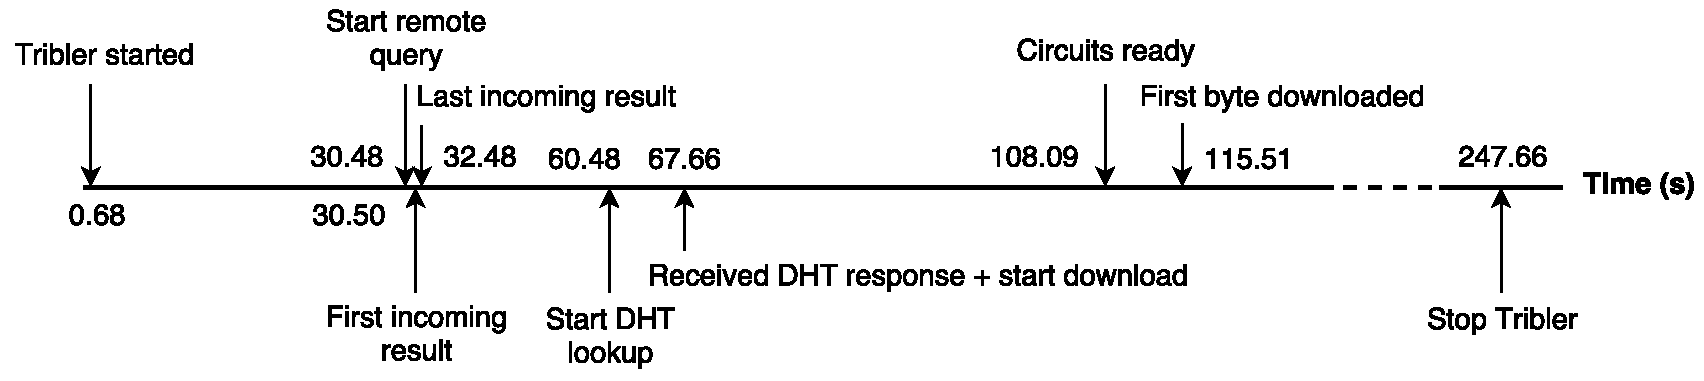
\includegraphics[width=1.0\columnwidth]{images/big_experiment/big_experiment_breakdown}
	\caption{A timeline of events during the runs. For each event, the average time is calculated across all runs.}
	\label{fig:big-experiment-breakdown}
\end{figure}

The average start-up time of Tribler during our experiments is 0.68 seconds. While this number is higher than the value as determined in Section \ref{sec:startup-experience} (0.35 seconds), it is still well under a second. The differences are most likely due to inequality in hardware specifications across the used machines.\\\\
After around 30 seconds, we have established enough peer connections in the \emph{SearchCommunity}, and we perform a remote keyword search. We notice that the first incoming response is very fast: on average, it arrives after 20 milliseconds, which is significantly faster than the value determined in Section \ref{sec:remote-content-search-experiment} (260 milliseconds). We believe this is explained due to the fast Internet connection of the DAS5 supercomputer. The last response takes on average 2.0 seconds to arrive, which is comparable to the value determined in \ref{sec:remote-content-search-experiment} (2.1 seconds).\\\\
Exactly 30 seconds after performing our remote search, we schedule our five DHT lookups if we received search results. On average, it takes 7.16 seconds for our DHT lookup to be completed, which is slightly slower than the average lookup time we found during the experiment in Section \ref{subsec:dht-experiment} (5.81 seconds). We do not have a solid explanation for this difference, other than that we are considering different torrents. After we received the first meta info response, we immediately start the download associated with the torrent of the received meta info.\\\\
After the anonymous download has started, Tribler attempts to build circuits which takes on average 40.43 seconds to complete. This seems a long time if we consider that Tribler has been running for several minutes and should have a sufficient amount of peers in the community responsible for managing circuits. To better understand the circuit building logic, we create an ECDF to get an overview of the distribution of time until our anonymous connections are ready, see Figure \ref{fig:big-experiment-circuits}.\\

\begin{figure}[!h]
	\centering
	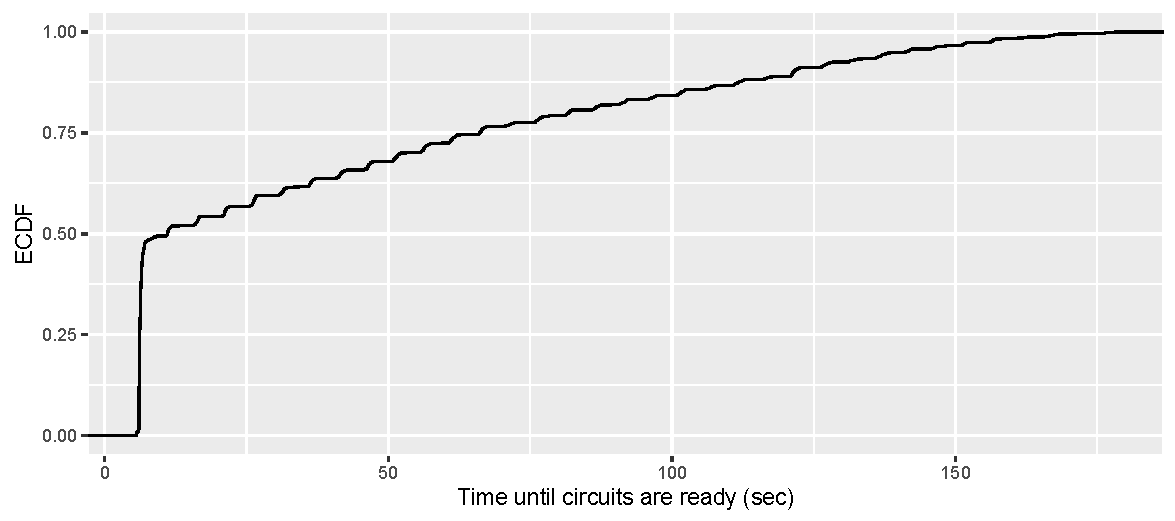
\includegraphics[width=1.0\columnwidth]{images/big_experiment/circuits_ecdf}
	\caption{An ECDF of the time until the circuits are ready.}
	\label{fig:big-experiment-circuits}
\end{figure}

We note that just under 50\% of the circuits are built within seven seconds. For runs where circuits are taking a longer time to be ready, we notice a step-like pattern which can be explained by the fact that we are building circuits at fixed time intervals (five seconds). Some circuits can even take several minutes to built. Figure \ref{fig:big-experiment-circuits} shows that the circuit built time can be improved, for instance, we might try to create additional circuits, more than we need in case the creation of circuits times out or fails due to other reasons.\\\\
After the circuits are built, it takes 7.42 seconds on average before we received our first byte, which might be slightly but not significantly slower than the times observed when performing a non-anonymous download. We address some of this increase in time to our implemented workaround to start the download and to the overhead caused by the anonymous overlay network.

\section{Integration in Jenkins}
The experiment described in this Section gave us insights in the failures and duration of various operations commonly performed by users in Tribler. In combination with the scenario file mechanism as described in Section \ref{sec:environment-specifications}, we can create a Jenkins job that performs the experiment as described in this Section to give developers feedback about the consequences of their modifications on the operation of core operations. This job can be executed parallel during the testing phase displayed in Figure \ref{fig:jenkins-pipeline}. We should change the structure of the experiment to have a better success rate, for instance, by searching for and downloading torrents with a good swarm health.\\\\
Due to time constraints, we were not able to implement this feature, however, there are no major technical obstacles.
